\subsection{Ca sử dụng xem ảnh theo khuôn mặt}

\vspace{0.5cm}

\noindent 
\begin{tabularx}{\linewidth}{| l | X |} 
\hline 
\textbf{Mô tả} & Người dùng muốn xem danh sách các ảnh gốc mà 1 khuôn mặt được phân loại chứa. \\
\hline 
\textbf{Luồng cơ bản} & 1. Người dùng chọn khuôn mặt muốn xem danh sách ảnh. \newline
                       2. Hệ thống lấy danh sách ảnh chứa khuôn mặt được chọn . \newline
                       3. Hệ thống nhóm ảnh theo ngày đăng. \newline
                       5. Hệ thống hiển thị giao diện với tên khuôn mặt và danh sách ảnh được sắp xếp dạng lưới. \\
\hline 
\textbf{Hậu điều kiện} & - Người dùng có thể chọn ảnh để xem chi tiết. \newline
                          - Người dùng có thể đổi tên khuôn mặt. \\
\hline 
\textbf{Yêu cầu phi chức năng} & -Hệ thống xử lý lấy dữ liệu danh sách ảnh không quá 2s. \\
\hline 
\end{tabularx}

\vspace{0.8cm}

\noindent 
\begin{tabular}{| c | c |}
    \hline
    \textbf{Biểu đồ hoạt động} & \textbf{Quan hệ} \\ 
    \hline
    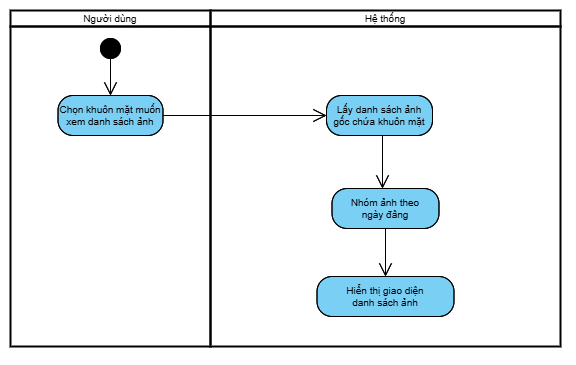
\includegraphics[width=0.6\linewidth]{figures/c3/3-3-11-activity-diagram.png} 
    &  
    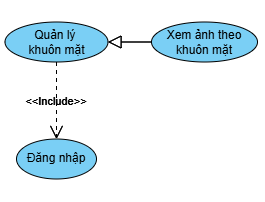
\includegraphics[width=0.35\linewidth]{figures/c3/3-3-11-relationship.png} \\ 
    \hline
\end{tabular}

\begin{figure}[H]
    \centering  
    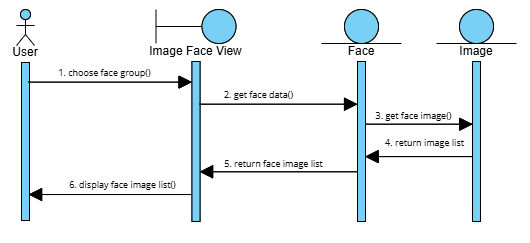
\includegraphics[width=1\textwidth]{figures/c3/3-3-11-sequence-diagram.png}
    \caption{Biểu đồ tuần tự ca sử dụng xem ảnh theo khuôn mặt.}
    \label{fig:3-3-11-sequence-diagram}
\end{figure}